\documentclass{jsarticle}
\usepackage[margin = .7in]{geometry}
\usepackage[dvipdfmx]{graphicx}
\usepackage{listings}
\usepackage{amsmath}
\usepackage{bm}
\usepackage{ascmac}
\usepackage[dvipdfmx]{hyperref}
\lstset{%
  language={python},
  basicstyle={\small},%
  identifierstyle={\small},%
  commentstyle={\small\itshape},%
  keywordstyle={\small\bfseries},%
  ndkeywordstyle={\small},%
  stringstyle={\small\ttfamily},
  frame={tb},
  breaklines=true,
  columns=[l]{fullflexible},%
  numbers=left,%
  xrightmargin=0zw,%
  xleftmargin=3zw,%
  numberstyle={\scriptsize},%
  stepnumber=1,
  numbersep=1zw,%
  lineskip=-0.5ex%
}

\begin{document}
\title{卒論テーマ候補 :複数均衡}
\author{池上 慧}
\maketitle

\section{やってみたこと}
Seim (2006)のような不完備情報の参入モデルでの複数均衡の取り扱いを調べてみました。ソースコードは\href{https://github.com/keiikegami/multiplicity}{ここ}にあります。

擬似データとして、以下のようなデータを作成するコードを書きました。
\begin{center}
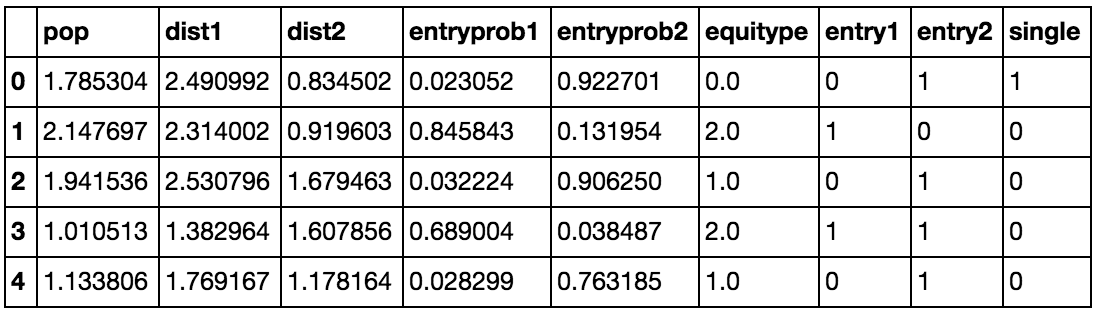
\includegraphics[width=10cm]{table1.png}
\end{center}
データの作成に関してのnotebookは\href{https://github.com/keiikegami/multiplicity/blob/master/sample_data_generation.ipynb}{こちら}にあります。

ここで行はサンプルとして得られている市場を、popは人口、dist1が企業1のコストを、dist2が企業2のコスト、entryprobはそれぞれの市場でモデルの均衡が与える参入確率のうち選択されたもの、equitypeは0が一つしか均衡がないことを1が複数均衡が存在した時に安定的な均衡のうちの片方が選ばれたこと、2はその逆の均衡が選ばれたことをそれぞれ示しています。singleは一つしかモデルに均衡が存在しないことを示すダミー変数です。結果として各企業が参入したか否かはentry1とentry2でダミー変数として表示されています。



























\end{document}
